%-------------------------------------------------------------------------------
\section{Results}
\label{sec:results}
%-------------------------------------------------------------------------------

\begin{figure}[t]
\centering
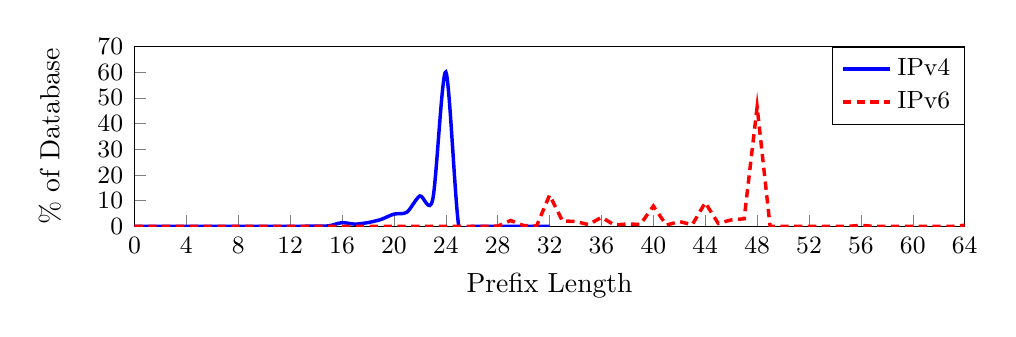
\begin{tikzpicture}
    \large
    \begin{axis}[
        xlabel=Prefix Length,
        ylabel=\% of Database,
        xmin=0, xmax=64,
        ymin=0, ymax=70,
        xtick={0,4,...,64},
        ytick={0,10,...,70},
        width=\columnwidth,
        height=110pt,
        xticklabel style={rotate=0,font=\small},
        yticklabel style={rotate=0,font=\small},
        xlabel style={font=\normalsize,at={(axis description cs:.5,-.2)}},
        ylabel style={font=\normalsize,at={(axis description cs:-.075,.5)}},
        legend style={at={(1,1)},anchor=north east,font=\small},
        tick pos=left
    ]
    \addplot[line width=1.25pt,mark=none,smooth,color=blue]
    plot coordinates {
        (0,0)
        (10,0)
        (11,0.01)
        (12,0.03)
        (13,0.06)
        (14,0.13)
        (15,0.23)
        (16,1.45)
        (17,0.89)
        (18,1.49)
        (19,2.7)
        (20,4.78)
        (21,5.54)
        (22,11.84)
        (23,10.68)
        (24,60.07)
        (25,0.08)
        (26,0)
        (32,0)
    };
    \addlegendentry{IPv4}
    \addplot[line width=1.25pt,mark=none,densely dashed,color=red]
    plot coordinates {
        (0,0)
        (19,0)
        (20,0.01)
        (21,0)
        (22,0)
        (23,0)
        (24,0.02)
        (25,0)
        (26,0.01)
        (27,0.01)
        (28,0.11)
        (29,2.31)
        (30,0.32)
        (31,0.16)
        (32,12.17)
        (33,2.07)
        (34,1.96)
        (35,0.69)
        (36,3.53)
        (37,0.57)
        (38,0.94)
        (39,0.77)
        (40,7.91)
        (41,0.51)
        (42,1.9)
        (43,0.65)
        (44,9.27)
        (45,1.16)
        (46,2.54)
        (47,2.97)
        (48,46.48)
        (49,0.01)
        (50,0)
        (51,0)
        (52,0.03)
        (53,0)
        (55,0)
        (56,0.44)
        (57,0)
        (63,0)
        (64,0.46)
    };
    \addlegendentry{IPv6}
    \end{axis}
\end{tikzpicture}
\vspace{-0.5em}
\caption{IPv4 and IPv6 prefix length distributions in AS65000 and AS131072, respectively, for September 2023}
\label{fig:bgp_dist}
\vspace{-\baselineskip}
\end{figure}

In this section, we introduce the databases, target implementations, and parameter values that we selected for our experiments. We use the \cram metrics to determine the best IPv4 (\resail) and IPv6 (\bsic) algorithms {\em before} implementation. We then compare the resource utilizations of the best \cram algorithms with those of state-of-the-art IP lookup schemes {\em after} implementation.

\subsection{Databases} \label{subsec:databases}

For IPv4, we used the AS65000 BGP routing table (Sep. 2023)~\cite{cidr_report_ipv4} which has close to 930k IPv4 prefixes. For IPv6, we used the AS131072 BGP routing table (Sep. 2023)~\cite{cidr_report_ipv6} which has close to 190k IPv6 prefixes. \cref{fig:bgp_dist} shows their prefix length distributions. We identify three key patterns:

{\bf P1.} Prefix distributions have major and minor spikes. For IPv4, there is a major spike at length 24 and minor spikes at lengths 16, 20, and 22. For IPv6, there is a major spike at length 48 and minor spikes at lengths 28, 32, 36, 40, and 44.

{\bf P2.} The majority of IPv4 prefixes are longer than 12 bits.

{\bf P3.} The majority of IPv6 prefixes are longer than 28 bits.

\subsection{Target Implementations} \label{subsec:target_implementations}

We obtained results for two different targets: an ideal RMT chip and Intel Tofino-2 (also RMT). Since RMT is a stricter variant of dRMT with additional access restrictions, we expect our RMT results to be reproducible on a dRMT chip.

{\bf Ideal RMT Chip (Simulation):} We define an ideal RMT chip to be an RMT chip with Tofino-2 specifications (same memory, number of stages, etc.)~\cite{bf_p4c} that can achieve 100\% SRAM utilization and perform at least two dependent ALU operations per stage. The resource utilization for an ideal RMT chip is obtained through simulation by using Tofino-2 SRAM page~(128x1024b) and TCAM block~(44x512b) sizes. If the number of TCAM blocks or SRAM pages used by a table exceeds the amount available in a MAU~(stage), the table is simply partitioned across multiple MAUs. Since Tofino-2 has 20 MAUs, results that require over 20 are considered infeasible.

% The number of TCAM blocks required per table is given by $x*y$ where $x$ is the ceiling of $TableWidth/BlockWidth$ and $y$ is the ceiling of $TableDepth/BlockDepth$. The number of SRAM pages required per table is given by the ceiling of $(TableWidth*TableDepth)/(PageWidth*PageDepth)$.

{\bf Intel Tofino-2 (Implementation):} The resource utilization for Tofino-2 is obtained through implementation. We implement the best \cram algorithms using P4 and compile them with the Intel P4 compiler. P4 Insight~\cite{p4_insight} then outputs detailed resource mappings and visualizations specific to Tofino-2.

\subsection{Parameter Values} \label{subsec:parameters}

We choose parameter values based on observations from \cref{subsec:databases}.

\resail's key parameter is $min\_bmp$, the smallest bitmap available. We choose $min\_bmp=13$ because there are so few IPv4 prefixes shorter than 13 bits {\bf (P2)}, thus minimizing the amount of prefix expansion needed.

\bsic's key parameter is $k$, the initial slice size. As recommended by \cite{dxr}, for IPv4, we choose $k=16$. For IPv6, we choose $k=24$ because most IPv6 prefixes are longer than 28 bits {\bf (P3)}. Therefore, a $k$ value that is close to but smaller than 28 can compress over 190k prefixes into just 7k TCAM entries. We briefly explore other choices of $k$ for IPv6 and examine potential latency-memory trade-offs in \cref{subsec:tradeoff}.

\mashup's key parameter is its set of strides. Intuitively, we want to select strides that mirror the distribution spikes {\bf (P1)} seen in \cref{fig:bgp_dist} because they will minimize prefix expansion. For IPv4, we choose 16-4-4-8~(spikes at 16, 20, 24). For IPv6, we choose 20-12-16-16~(spikes at 32, 48). We do not select 32 as the first stride because it is too wide---especially for the root node which may contain many entries. Therefore, we decompose 32 into separate strides of 20 and 12.

\subsection{Comparisons {\em before} Implementation} \label{subsec:before_implementation}

\begin{table}[t]
    \centering
    \small
    \setlength\extrarowheight{1.25pt}
    \setlength\tabcolsep{2.5pt}
    \begin{tabular}{lccc}
    \hline
      \thead[l]{Scheme} & \thead[c]{TCAM Bits} & \thead[c]{SRAM Bits} & \thead[c]{Steps} \\ 
        \hline
        \mashup (16-4-4-8) & 0.31 MB & 5.92 MB & 4 \\
        \bsic ($k$=16) & 0.07 MB & 8.64 MB & 10 \\
        \resail ($min\_bmp$=13) & 3.13 KB & 8.58 MB & 2 \\
        \bottomrule
    \end{tabular}
    \vspace{-0.5em}
    \caption{\cram metrics for IPv4 prefixes in AS65000}
    \label{tab:cram_ipv4}
    \vspace{-0.5em}
\end{table}

\begin{table}[t]
    \centering
    \small
    \setlength\extrarowheight{1.25pt}
    \setlength\tabcolsep{2.5pt}
    \begin{tabular}{lccc}
    \hline
      \thead[l]{Scheme} & \thead[c]{TCAM Bits} & \thead[c]{SRAM Bits} & \thead[c]{Steps} \\ 
        \hline
        \mashup (20-12-16-16) & 0.32 MB & 0.77 MB & 4 \\
        \bsic ($k$=24) & 0.02 MB & 3.18 MB & 14 \\
        \bottomrule
    \end{tabular}
    \vspace{-0.5em}
    \caption{\cram metrics for IPv6 prefixes in AS131072}
    \label{tab:cram_ipv6}
    \vspace{-\baselineskip}
\end{table}

Recall that \cram metrics enable quick estimation of algorithm scalability {\em before} implementation.

We present IPv4 and IPv6 \cram metrics in \cref{tab:cram_ipv4} and \cref{tab:cram_ipv6}, derived from the optimization steps in \cref{subsec:designing_resail}, \cref{subsec:designing_bsic}, and \cref{subsec:designing_mashup}, for the IPv4 and IPv6 BGP tables, respectively.

For IPv4, \resail outperforms \bsic in all three \cram metrics. Between \resail and \mashup, \resail wins in TCAM and steps but loses in SRAM. However, \mashup requires 100X more TCAM than \resail, whereas \resail requires only 1.4X more SRAM than \mashup. Therefore, we determine \resail to be the best \cram IPv4 algorithm.

For IPv6, we choose between \bsic and \mashup. \bsic wins in TCAM but loses in SRAM and steps. \mashup requires 16X more TCAM than \bsic, while \bsic requires roughly 4X more SRAM and steps than \mashup. As before, we prioritize TCAM because it is more expensive and limited than SRAM---for example, Tofino-2 contains 19X more SRAM than TCAM. Although \bsic uses more steps than \mashup, this is due to \bsic's use of BSTs, which have a high initial step cost. Therefore, we determine \bsic to be the best \cram IPv6 algorithm {\em for Tofino-2}. However, for more stage-constrained ASICs, \mashup is likely better.

\begin{table}[t]
    \centering
    \small
    \setlength\extrarowheight{1.25pt}
    \setlength\tabcolsep{2.5pt}
    \begin{tabular}{lccc}
    \hline
      \thead[l]{Scheme} & \thead[c]{TCAM Blocks} & \thead[c]{SRAM Pages} & \thead[c]{Stages} \\ 
        \hline
        \mashup (16-4-4-8) & 235 & 216 & 10 \\
        \bsic ($k$=16) & 74 & 558 & 16 \\
        \resail ($min\_bmp$=13) & 2 & 556 & 9 \\
        \bottomrule
    \end{tabular}
    \vspace{-0.5em}
    \caption{Ideal RMT mapping for IPv4 prefixes in AS65000}
    \label{tab:ideal_rmt_ipv4}
    \vspace{-0.5em}
\end{table}

\begin{table}[t]
    \centering
    \small
    \setlength\extrarowheight{1.25pt}
    \setlength\tabcolsep{2.5pt}
    \begin{tabular}{lccc}
    \hline
      \thead[l]{Scheme} & \thead[c]{TCAM Blocks} & \thead[c]{SRAM Pages} & \thead[c]{Stages} \\ 
        \hline
        \mashup (20-12-16-16) & 178 & 47 & 8 \\
        \bsic ($k$=24) & 15 & 211 & 14 \\
        \bottomrule
    \end{tabular}
    \vspace{-0.5em}
    \caption{Ideal RMT mapping for IPv6 prefixes in AS131072}
    \label{tab:ideal_rmt_ipv6}
    \vspace{-\baselineskip}
\end{table}

To verify the validity of the \cram metrics, we explicitly map each \cram algorithm to an ideal RMT chip and present its resource utilization in \cref{tab:ideal_rmt_ipv4} and \cref{tab:ideal_rmt_ipv6}. This mapping, which accounts for Tofino-2 TCAM block sizes, SRAM page sizes, and per-stage memory, is precisely the complicated process that the \cram model seeks to relieve algorithm designers of. Comparing \cref{tab:cram_ipv4} with \cref{tab:ideal_rmt_ipv4} and \cref{tab:cram_ipv6} with \cref{tab:ideal_rmt_ipv6}, observe that the \cram metrics accurately predict a target algorithm's resource utilization and potential scalability.

\subsection{Comparisons {\em after} Implementation}
\label{subsec:after_implementation}

The previous subsection compared our three new algorithms {\em before} implementation using \cram metrics. Here, we compare the best \cram algorithms {\em after} implementation on Tofino-2 against the best pre-existing IPv4 and IPv6 schemes.

\subsubsection{Baseline Selection} \label{subsubsec:baselines}

We select four single-resource baselines: SRAM-only for IPv4 and IPv6, and TCAM-only for IPv4 and IPv6.

{\bf SRAM-only for IPv4:} We choose \sail~\cite{sail} as our SRAM-only IPv4 baseline due to its on-chip memory bound for short prefixes, which enables it to scale very well. Although IPv4 schemes like Poptrie~\cite{poptrie} and \dxr~\cite{dxr} use less memory, they require too many memory accesses and stages.

{\bf SRAM-only for IPv6:} We choose \hibst~\cite{hibst} as our SRAM-only IPv6 baseline because it is the most memory-efficient IPv6 lookup algorithm to date~\cite{xoroffsettrie}. It uses a treap data structure that maps each prefix to a unique node.

{\bf TCAM-only for IPv4 and IPv6:} We choose a logical TCAM as our TCAM-only IPv4 and IPv6 baseline because, although TCAM-oriented schemes exist for reducing power consumption~\cite{liu} or merging multiple FIBs~\cite{virtual_routers}, none focus on scaling IP lookup for a single database.

\begin{table}[t]
    \centering
    \small
    \setlength\extrarowheight{1.25pt}
    \setlength\tabcolsep{2.5pt}
    \begin{tabular}{lcccc}
    \hline
      \thead[l]{Scheme} & \thead[c]{TCAM \\ Blocks} & \thead[c]{SRAM \\ Pages} & \thead[c]{Stages} & \thead[c]{Target Chip} \\ 
        \hline
        \resail ($min\_bmp$=13) & 17 & 750 & 16 & Tofino-2 \\
        \resail ($min\_bmp$=13) & 2 & 556 & 9 & Ideal RMT \\
        \sail & - & 2313 & 33 & Ideal RMT \\
        Logical TCAM & 1822 & - & 76 & Ideal RMT \\
        Tofino-2 Pipe Limit & 480 & 1600 & 20 & - \\
        \bottomrule
    \end{tabular}
    \vspace{-0.5em}
    \caption{Baseline comparison for IPv4 prefixes in AS65000}
    \label{tab:after_implementation_ipv4}
    \vspace{-0.5em}
    % \vspace{-\baselineskip}
\end{table}

\begin{table}[t]
    \centering
    \small
    \setlength\extrarowheight{1.25pt}
    \setlength\tabcolsep{2.5pt}
    \begin{tabular}{lcccc}
    \hline
      \thead[l]{Scheme} & \thead[c]{TCAM \\ Blocks} & \thead[c]{SRAM \\ Pages} & \thead[c]{Stages} & \thead[c]{Target Chip} \\ 
        \hline
        \bsic ($k$=24) & 15 & 416 & 30 & Tofino-2 \\
        \bsic ($k$=24) & 15 & 211 & 14 & Ideal RMT \\
        \hibst & - & 219 & 18 & Ideal RMT \\
        Logical TCAM & 762 & - & 32 & Ideal RMT \\
        Tofino-2 Pipe Limit & 480 & 1600 & 20 & - \\
        \bottomrule
    \end{tabular}
    \vspace{-0.5em}
    \caption{Baseline comparison for IPv6 prefixes in AS131072}
    \label{tab:after_implementation_ipv6}
    \vspace{-\baselineskip}
\end{table}

\subsubsection{IPv4 Comparison} \label{subsubsec:ipv4_comparison}

\cref{tab:after_implementation_ipv4} compares the ideal RMT resource utilization of \resail with the IPv4 baselines. \resail requires 911X fewer TCAM blocks than the logical TCAM and approximately 4X fewer SRAM pages and stages than \sail. Although \sail's memory scales efficiently, its high upfront cost makes it impractical for RMT-like chips. \resail outperforms the logical TCAM, which only supports IPv4 databases of up to 245,760 entries---about 3.8X smaller than the current IPv4 BGP table.

\cref{tab:after_implementation_ipv4} also compares \resail on an ideal RMT chip and on Tofino-2. While \resail fits on Tofino-2 for AS65000, it requires nearly 1.4X more SRAM pages and 2X more stages than on an ideal RMT chip. This is because Tofino-2 reserves bits in each SRAM word for identifying actions, limiting the maximum SRAM utilization to 50\%. The increase in TCAM is due to extra ternary bitmask tables needed for extracting bits.

\subsubsection{IPv6 Comparison} \label{subsubsec:ipv6_comparison}

\cref{tab:after_implementation_ipv6} compares the ideal RMT resource utilization of \bsic with the IPv6 baselines. \bsic uses less SRAM and fewer stages than \hibst, at the cost of 15 TCAM blocks. Both \bsic and \hibst support the current IPv6 BGP table, whereas the logical TCAM only supports up to 122,880 entries---about 1.6X smaller than the current IPv6 BGP table.

\cref{tab:after_implementation_ipv6} also compares \bsic on an ideal RMT chip and on Tofino-2. Our ideal RMT chip assumes each stage can perform at least two dependent ALU operations. However, in practice, a Tofino-2 stage can execute only one level of ALU logic. Consequently, each BST level requires two stages: one for comparing the search key and another for performing the P4 action. This creates a repeating pattern where an SRAM-intensive stage is followed by a stage with minimal SRAM usage. Although \bsic on Tofino-2 requires 30 stages (ten over the Tofino-2 pipe limit), we successfully fit \bsic for AS131072 by recirculating each packet. However, this effectively halves the number of available switch ports.